\section{General radiation pressure modeling}


\subsection{Mechanics of radiation pressure}
\label{subsec:general-rp-mechanics}

\gls{RP} results from the momentum transfer between electromagnetic radiation and a surface. A spacecraft may receive such radiation from the Sun but also from other celestial bodies: planets and moons emit albedo radiation through reflection of sunlight and thermal radiation depending on surface temperature. The \gls{RP} exerts a force on the spacecraft governed by surface properties such as area, reflectivity and absorptivity. The resulting acceleration is the result of a complex interplay of the bodies emitting radiation (the "sources") and the spacecraft receiving the radiation (the "target").

Radiation can characterized by the radiant flux density, which commonly has units of \unit{\irr}. Radiosity is the \emph{emitted and reflected} radiant flux density of an opaque surface. The irradiance $E$ is the \emph{incident} radiant flux density on a surface and provides a convenient way to decouple source and target models: the irradiance and the direction of incidence are sufficient to determine the target acceleration, independent of the actual source. We can combine this information into a vector quantity which we call directional irradiance $\vb E = E \vu r_{t/s}$, where $\vu r_{t/s}$ is the unit vector in the source--to--target direction. One or more directional irradiances, which can be though of as light rays, are the output of a source model and used as input to the target model. The \gls{RP} exerted on an irradiated surface is proportional to $1/c$, where $c = \qty{299792458}{m/s}$ is the speed of light. Given the magnitude of $c$, \gls{RP} is usually small (around \qty{4.5e-6}{\N\per\m\squared} for solar radiation at Earth, where $E=\qty{1361}{\irr}$~\cite{Kopp2011}).

Electromagnetic radiation is often composed not just of a single wavelength but rather a range of wavelengths. The distribution can be described by the spectral irradiance in units of \unit{\W\per\square\m\per\Hz}. Since surface properties are often wavelength-dependent, the target model would also have to be aware of the distribution. However, the surface properties as a function of wavelength are often not known, which is also the case for \gls{LRO}. Therefore, we assume the irradiance from source models to be integrated over the whole spectrum and the surface properties of the target model to be valid for all wavelengths.




\subsection{Reflectance distribution}
\label{subsec:general-reflectance-distribution}

Describing the reflectance of a surface is key to \gls{RP} modeling. Both the way a source reflects sunlight and the direction a target is accelerated in depend on the angular distribution of reflectance.

\subsubsection{General reflectance distribution}
In general, reflectance comprises a diffuse (scattered in many directions) and a specular (mirror-like) component. The remaining energy is absorbed by the surface. The reflectance varies with surface normal $\vb N$, incoming radiation direction $\vb L$, and observer direction $\vb V$. This geometry is shown in \cref{fig:reflection-geometry}. A \gls{BRDF} describes the fraction of irradiance reflected towards the observer per steradian, i.e.~\cite{Wetterer2014}
\begin{align}
    f_r (\theta_i, \phi_i, \theta_r, \phi_r)
    = \frac{dL_r(\theta_r, \phi_r)}
    {dE_i(\theta_i, \phi_i)},
\end{align}
where $dL_r$ is the reflected radiance (the directional counterpart to radiosity, typically in \unit{\W\per\square\m\per\steradian}) and $dE_i$ is the received irradiance.

\begin{figure}[t]
    \centering
    \includegraphics[width=0.8\linewidth]{figures/reflection_geometry.ai}
    \caption{Geometry of a \gls{BRDF} for a surface with normal $\vb N$, incoming direction $\vb L$, and observer direction $\vb V$ (adapted from \cite{Wetterer2014}).}
    \label{fig:reflection-geometry}
\end{figure}

The planetary surface \gls{BRDF} directly leads to the albedo irradiance received by a target if the sun irradiance at the planet surface and the solid angle subtended by the target are known.

The target surface \gls{BRDF} gives the direction in which the target is accelerated through integration over all directions $\vb V$ in which radiation is reflected. The unitless reaction vector, which includes both the direction and magnitude based on absorped, specularly and diffusely reflected fractions, is therefore~\cite{Wetterer2014}
\begin{align}
    \label{eq:brdf-reaction-general}
    \vb R = -\left[ \vb L + \int_{0}^{2\pi} \int_{0}^{\pi/2} f_r \cos\theta_r \vb V d\theta_r d\phi_r \right].
\end{align}
This vector encapsulates the mechanics of momentum transfer. The reaction is minimal for pure absorption ($f_r = 0$). The reaction is maximal (double the minimum) for pure specular reflection in the incidence direction.

\subsubsection{Specular--diffuse reflectance distribution}
A simplified \gls{BRDF} is usually more practical for \gls{RP} modeling: the reflectance is assumed to be a mix of an ideal Lambertian diffuse component and a purely mirror-like specular components. Such a \gls{BRDF} is given by~\cite{Wetterer2014}
\begin{align}
    \label{eq:brdf-specular-diffuse}
    f_r = C_d \frac{1}{\pi} + C_s \frac{\delta(\vb V - \vb M)}{\cos \theta_i}
\end{align}
where $C_d$ and $C_s$ are the diffuse and specular reflectivity coefficients. Together with the absorption coefficient $C_a$, energy is conserved when $C_a + C_d + C_s = 1$. The vector $\vb M = 2\cos\theta_i\vb N - \vb L$ is the direction of $\vb L$'s mirror-like reflection, which only contributes if $\vb V = \vb M$.

For this simplified \gls{BRDF}, the integral in \cref{eq:brdf-reaction-general} evaluates analytically to~\cite{Montenbruck2014}
\begin{align}
    \vb R = - \left[ (C_a + C_d) \vb L + \frac{2}{3} C_d \vb N + 2 \cos\theta_i C_s \vb N \right].
\end{align}
If the target is in thermodynamic equilibrium, all absorbed radiation will be reradiated instantaneously by Kirchhoff's law. If this reradiation is Lambertian, the reaction vector becomes~\cite{Montenbruck2014}
\begin{align}
    \vb R = - \left[ (C_a + C_d) \left(\vb L + \frac{2}{3} \vb N\right) + 2 \cos\theta_i C_s \vb N \right].
\end{align}
The specular contribution is strictly along the surface normal direction since its tangential components cancel. The Lambertian diffuse contribution (both reflected and reradiated) has a component along the incoming direction but also, weighted by a factor $2/3$ (see~\cite{Ziebart2004} for a derivation of this factor), a component along the surface normal. The reaction vector will thus always be in the plane spanned by $\vb L$ and $\vb N$.



\subsection{Radiation sources}
Radiation sources emit or reflect radiation, which exerts \gls{RP} onto the target. As explained in \cref{subsec:general-rp-mechanics}, the incident radiation at a target due to a source can be thought of as light rays, which are described by their directional irradiance at the target. How the directional irradiance is evaluated depends on the type of source.

\subsubsection{Isotropic point sources}
The simplest source model is a point source which isotropically radiates in all directions. This model is appropriate for far-away sources such as the Sun at \qty{1}{\astronomicalunit} distance. Due to the distance, all rays are effectively parallel and can be merged into a single ray, parallel to the source--to--target vector $\vb r_{t/s}$. For an isotropic source, the total luminosity $L$ (units of \unit{\W}) is uniformly distributed over a sphere, leading to an inverse square law. Therefore, the irradiance at the target is
\begin{align}
    \label{eq:irradiance-point-luminosity}
    E = \frac{L}{4\pi\norm{\vb r_{t/s}}^2}.
\end{align}
Alternatively, a reference irradiance $E_\text{ref}$, taken at a distance $\vb r_\text{ref}$ can be scaled:
\begin{align}
    E = E_\text{ref} \frac{r_\text{ref}}{\norm{\vb r_{t/s}}^2}.
\end{align}
The solar luminosity is \qty{3.828e26}{\W}~\cite{Prsa2016}, which corresponds to an irradiance of \qty{1361}{\irr} at \qty{1}{\astronomicalunit}. Note that these values are averages, which vary with the 11-year solar cycle by about \qty{0.1}{\percent} and more on shorter timescales due to sunspot darkening and facular brightening~\cite{Kopp2016}. Observational timeseries exist to account for these variations if necessary~\cite{Dewitte2017}.

\subsubsection{Paneled sources: Discretization}
Radiation due to planets and moons requires more involved source models. Planetary emissions comprise reflected solar radiation and thermal infrared radiation~\cite{Knocke1988}. The fraction of reflected sunlight is called albedo $a$; the corresponding type is therefore also called albedo radiation. Thermal radiation is due to absorbed solar energy that is re-emitted in a delayed fashion. Observation timeseries of albedo and thermal fluxes exist for Earth~\cite{Dewitte2017}, but physical modeling is required for the Moon.

Since planetary radiation is not isotropic and the spacecraft is typically much closer to the body than to the Sun, the source extent has to be considered. In contrast to the previously described point source, we therefore model Earth and Moon as extended sources. These are discretized into sub-sources, from which rays emanate that are, in general, not parallel. The sub-sources can be thought of as panels with an area, orientation, position, and radiosity model. The panel extent is captured by the area but any other panel properties are only evaluated at its center.

Different algorithms exist to divide the planet spheroid into panels. Some authors use a longitude--latitude grid (e.g.,~\cite{RodriguezSolano2011a,Woeske2019}, particularly with observed fluxes) or generate static, uniformly spaced panels over the whole sphere (e.g.,~\cite{Wetterer2014}). However, both approaches are inefficient for low-altitude spacecraft, which require a large number of panels, most of which are never visible. Therefore, the de-facto standard is the dynamic\footnote{Dynamic refers to the fact that panels move with the spacecraft, as opposed to static paneling, for which panels are invariant with spacecraft position or time.} paneling approach introduced by \citeauthor{Knocke1988}~\cite{Knocke1988}. The algorithm is described in more detail in~\cite{Knocke1989}.

% TODO expand: describe Knocke paneling in detail, with figure for zeta, beta...

In Knocke's approach, only the visible area of the planet is paneled. This area is a spherical cap centered at the subsatellite point and is divided into concentric rings which are divided into equal-area segments. A central panel is located at the subsatellite point. Each panel contributes to the irradiance received by the target. However, the effective area is projected by the viewing angle $\theta_r$ (see \cref{fig:reflection-geometry}) and the irradiance is attenuated by an inverse square law. In Knocke's approach, the rings are spaced such that each panel has the same projected, attenuated area. The projected, attenuated area $A'$ of a panel is defined as~\cite{Knocke1988}
\begin{align}
    A' = \frac{dA \cos \theta_r}{\norm{\vb r_{t/s}}^2},
\end{align}
where $dA$ is the geometric panel area and $r_{t/s}$ is the source--to--target vector. More rings and more panels per ring will improve the fidelity of the calculated irradiance, barring the resolution limit of the radiosity model (e.g., the albedo distribution). While arbitrary numbers of panels per ring are possible, Knocke suggests multiples of 6 (i.e., 6 panels in the first ring, 12 panels in the second ring, \dots).

\begin{figure*}[t]
    \centering

   \begin{subfigure}[c]{0.49\textwidth}
      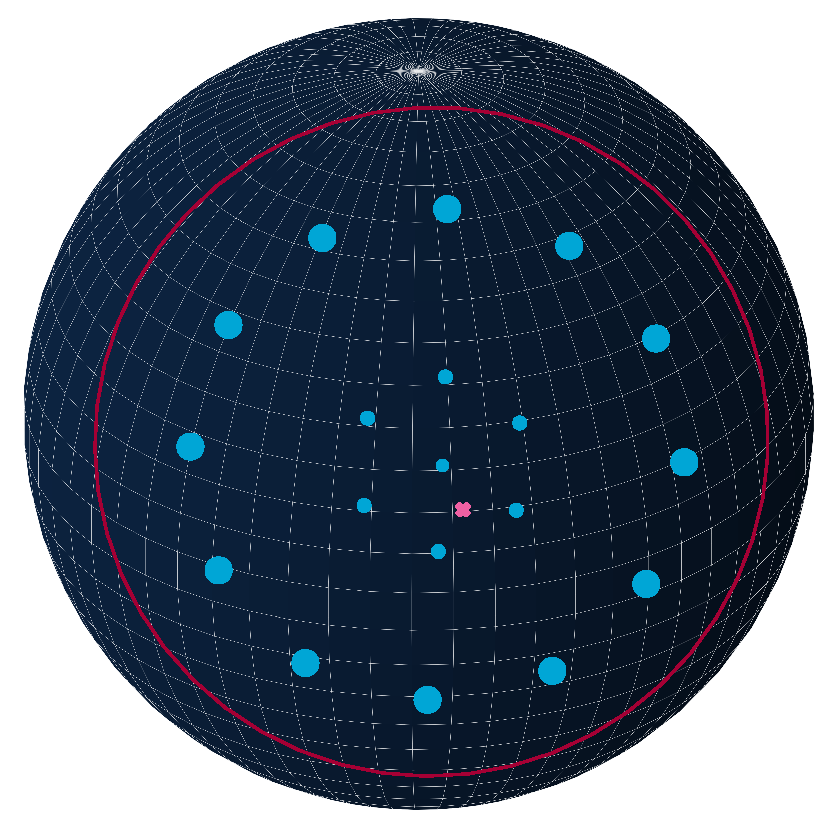
\includegraphics[width=\textwidth]{figures/plots/knocke_paneling_high.pdf}
      \subcaption{High altitude: $h = \qty{1500}{\km}$, 2 rings, angular diameter of cap = \ang{115}.}
      \end{subfigure}
   \hfill
   \begin{subfigure}[c]{0.49\textwidth}
      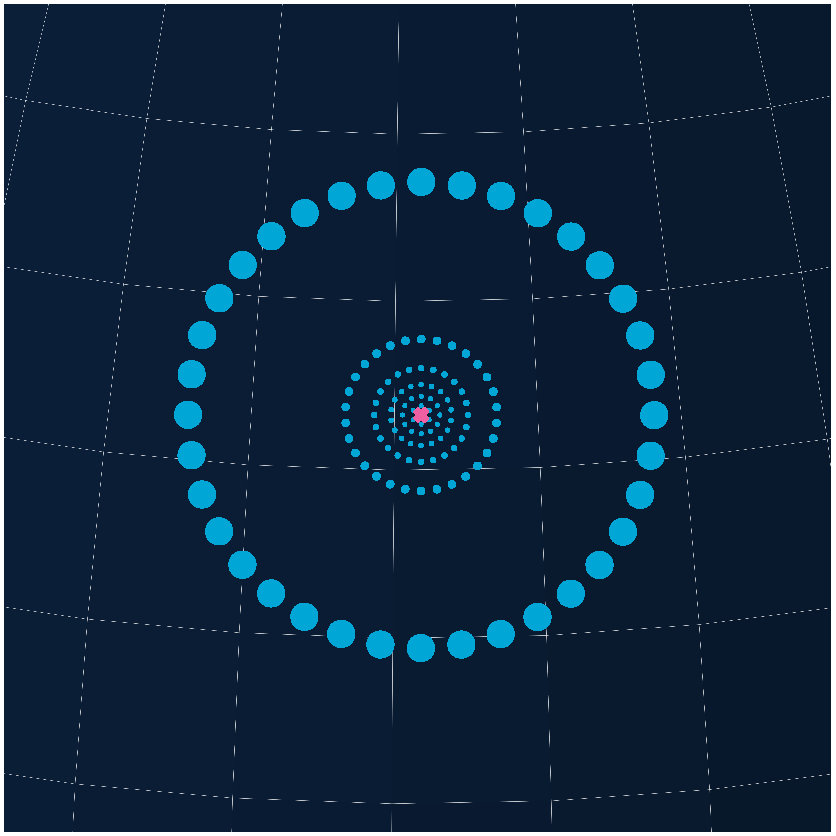
\includegraphics[width=\textwidth]{figures/plots/knocke_paneling_low.pdf}
      \subcaption{Low altitude: $h = \qty{50}{\km}$, 5 rings, angular diameter of cap = \ang{27}.}
   \end{subfigure}

   \caption{Panels generated with Knocke's dynamic approach for the Moon, which has a polar radius if \qty{1736}{\km}. The spacecraft (pink) sees a spherical cap (red), which contains rings of panels and is larger at higher altitudes $h$. Panel centers (light blue) are scaled proportional to the panel area. The panels have equal projected, attenuated areas and are therefore concentrated around the subsatellite point.}
   \label{fig:general-knocke-paneling}
\end{figure*}

Two examples at different spacecraft altitudes and with different ring numbers are shown in \cref{fig:general-knocke-paneling}. At higher altitudes, a larger area is visible (approaching a hemisphere for increasing altitudes) and panels are more uniform in area. At lower altitudes, the panels are more tightly spaced towards the subsatellite point and and panels increase in area towards the edge of the visible cap. This pattern is result of the equal projected, attenuated areas.

\subsubsection{Paneled sources: Radiosity models}
The emitted and reflected fluxes of a panel are described by a radiosity model. The irradiance at the target position can then be derived from the panel radiosity. Each panel can have one or more radiosity model, usually one for albedo radiation and one for thermal radiation. We will now present three such models.

The albedo radiosity model accounts for diffuse Lambertion reflection of solar radiation. It implements the specular--diffuse \gls{BRDF} from \cref{eq:brdf-specular-diffuse} with $C_s = 0$ and the albedo value $C_d = a$ at the panel center. The albedo radiosity of a panel is~\cite{Knocke1988}
\begin{align}
    \label{eq:radiosity-albedo}
    J_\text{albedo} = a \left(\cos\theta_i\right)_+ E_s,
\end{align}
where $E_s$ is the incoming solar irradiance at the panel (e.g., as found from \cref{eq:irradiance-point-luminosity}) and the angles are defined in \cref{fig:reflection-geometry}. The operator $(\cdot)_+$ restricts the input to positive values or zero otherwise.

The delayed thermal radiosity model assumes that absorbed radiation is emitted independently of incident solar radiation and the radiosity is thus not a function of $\theta_i$. The only spatial variations arise from emissivity differences. The emissivity of a surface is the ratio of the actual radiosity to the ideal black body radiosity. The delay arises from the planet's large thermal inertia. The delayed thermal radiosity of a panel is~\cite{Knocke1988}
\begin{align}
    \label{eq:radiosity-thermal-delayed}
    J_\text{thermal} = e \frac{E_s}{4},
\end{align}
where $e$ is the emissivity of the panel, evaluated at its center. The factor 1/4 is the ratio of absorbing area (a circle) to emitting area (a sphere).

The angle-based thermal radiosity model is more appropriate if the surface experience significant diurnal cooling and heating. The surface temperature is modeled as a function of the incidence angle and related to the radiosity through the Stefan--Boltzmann law. The surface temperature is interpolated between the minimum and maximum temperatures, $T_\text{min}$ and $T_\text{max}$ as
\begin{align}
    \label{eq:surface-temperature}
    T = \max\left( T_\text{max} \left(\cos\theta_i\right)_+^{1/4}, T_\text{min} \right).
\end{align}
The angle-based thermal radiosity of a panel is then~\cite{Lemoine2013}
\begin{align}
    \label{eq:radiosity-thermal-anglebased}
    J_\text{thermal} = e \sigma T^4
\end{align}
where $T$ is the surface temperature from \cref{eq:surface-temperature} at the panel center and $\sigma = \qty{5.670e-8}{\W\per\m\squared\per\K\tothe{4}}$ is the Stefan--Boltzmann constant. The maximum radiosity of $e \sigma T_\text{max}^4$ is usually larger than the near-constant $e E_s/4$ from \cref{eq:radiosity-thermal-delayed}, but quickly decreases as the panel moves away from the subsolar point (where $\theta_i = \ang{0}$). On the nightside, the thermal radiosity reduces to $e \sigma T_\text{min}^4$.

To obtain the irradiance at the target due to the panel radiosity, we assume that the emission follows Lambert's cosine law and account for the projected, attenuated area of the source panel. The irradiance then becomes
\begin{align}
    \label{eq:irradiance-from-radiosity}
    E = \left(\sum_{J_i \in \mathcal{J}} J_i\right) \frac{dA \left(\cos\theta_r\right)_+}{\pi\norm{\vb r_{t/s}}^2},
\end{align}
where $\mathcal{J}$ is any set of radiosity models, but usually the albedo model and one thermal model. Here, the source--to--target vector $\vb r_{t/s}$ uses the panel center position, not the source body center. The direction $\vu r_{t/s}$ of the corresponding directional irradiance $\vb E = E \vu r_{t/s}$  is therefore not the same for each panel and thus accounts for the extent of the source. The radiosity models in \cref{eq:irradiance-from-radiosity} can be summed since their irradiance emanates from the same point, the panel center. Note that, in general, the directional irradiances cannot be summed since the reflectance model of the target may be sensitive to the incoming direction of each ray. Therefore, a set of directional radiances $\mathcal{E}$ is handed to the radiation pressure target model for acceleration calculations.




\subsection{Radiation pressure targets}

depends on area, surface properties and mass

spacecraft thermal radiation pressure can be high
requires thermal model and knowledge of conductivity
therefore assume instantaneous reradiation

cannonball force always along source--target vector
paneled can have different force direction due to mix of specular and diffuse reflection

can sum directional irradiances for cannonball, but not for target



\subsection{Occultation}



